%% -----------------------------------------------------------------------------

A type-level mutation is {\em interesting\/} (1) if the type checker rejects the fully typed version of the mutant,
(2) running the mutant with all type annotations removed raises a run-time error, and
(3) that error's stack trace contains source locations from at least three modules.

Here is the rationale for these three conditions:
\begin{enumerate}

\item An impedance mismatch is a clash between the type ascription of one
module's imports and another module's exports. Hence, type checking should fail
for an interesting mutant.

\item The goal of a comparative evaluation is to give the rational programmer a
chance to debug the same scenario using different pieces of information.  In the
case of gradual typing semantics, a meta-theorem due to \citet{gf-icfp-2018} says that if a program raises an exception under
Erasure, it also errors under all other semantics.  Hence, a comparison of blame
information insists that an interesting mutant {\em raises a run-time exception
under Erasure\/}.

{\bf Note} While this choice favors Erasure over Transient and Natural and, for
the same reason, Transient over Natural, some form of bias towards one or the
other semantics is unavoidable. Tipping the scales in favor of the theoretically
weakest semantics yields the most stable results. 
Section~\ref{sec:discussion} includes some further discussion of this choice.


\item If the evaluation of a mutated module immediately raises an exception because
of the changes, there is no work for the rational programmer. Indeed, if the
stack trace contains source pointers to two modules, the scenario is still
uninteresting. Every ordinary benchmark program comes with a {\tt main} module
that acts as a driver, whose source is guaranteed to be included in the stack
trace.  Hence, the definition of interesting mutation insists on the presence of
three different modules in the stack trace. This guarantees that the debugging
scenario demands a sufficiently sophisticated effort, due to the interaction
between the buggy module with its context.  In these cases, the rational
programmer must contend with at least two modules involved in a faulty
interaction.

\end{enumerate}

\begin{figure}
 \centering
 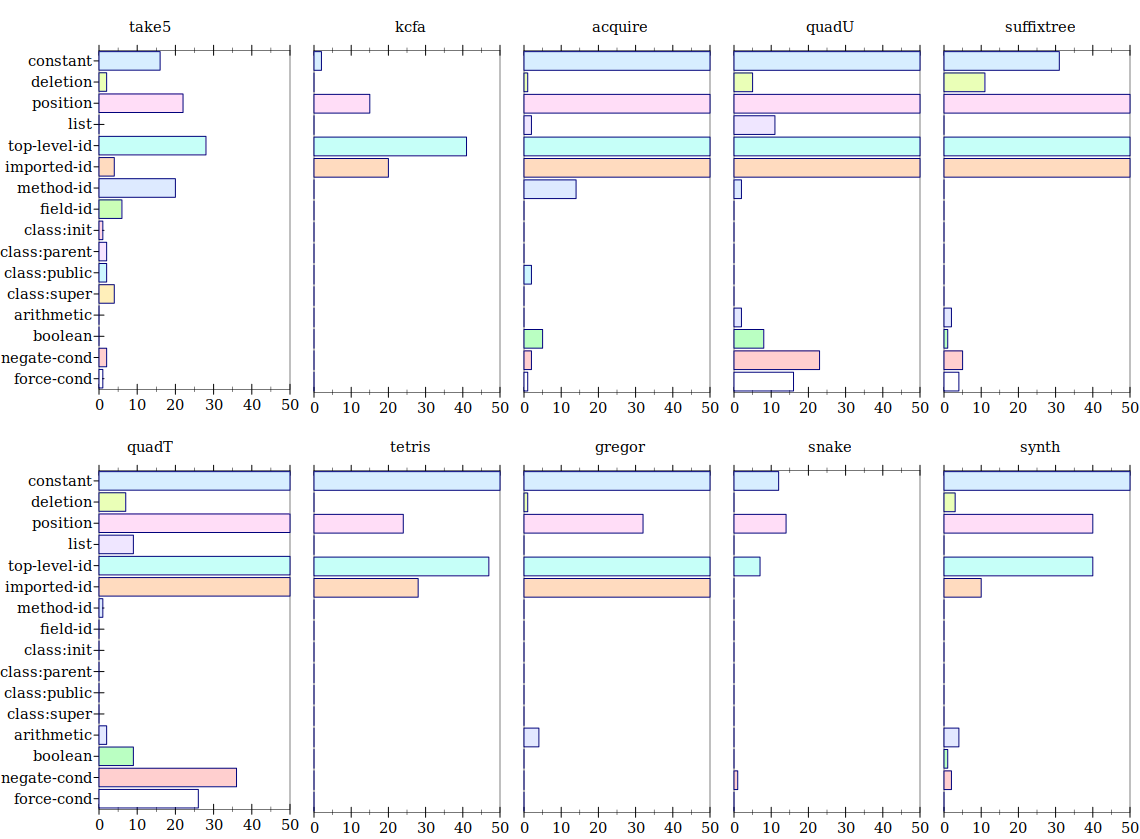
\includegraphics[scale=0.33]{./plots/mutant-breakdown}

 \vspace{1em}

 \begin{minipage}{\textwidth}
 Each plot shows a breakdown of interesting mutants by mutator.
 Each mutator corresponds to a bar representing the number of interesting mutants generated by that mutator.
 The counts are cut off at 50, so those bars reaching the edge of the plot represent 50 or more interesting mutants.
 \end{minipage}

\caption{Breakdown of interesting mutants by mutator, per benchmark.}
 \label{fig:mutant-breakdown}
\end{figure}

The definition of interesting mutants creates a powerful filter. All
together, the listed mutators produce 16,800 interesting mutants across all benchmarks; see
figure~\ref{fig:mutant-breakdown} for an overview. Broken down by benchmark, the
mutators produce at least 40 interesting mutants for every benchmark, and
these mutants originate from at least four different mutators per benchmark.
Thus, the mutators result in a sizable and diverse population of scenarios for
every benchmark.  Furthermore, every mutator contributes interesting mutants in at least
one benchmark.  Some mutators apply only to a few benchmarks, because they
target rather specific features; for instance, the class-focused mutators are
mainly effective in a program that makes extensive use of object-oriented
features.

The goal of filtering for interesting mutants guided countless iterations of
adding, removing, and refining mutators in table~\ref{table:mutation-ops}.  For
an illustrative example, consider a candidate mutator that casts the tests of
conditionals to the {\tt Any} type. Like the example explained at the end of the
preceding subsection, this mutant would suppress occurrence typing. But, it
would not be interesting because an execution would not raise a run-time error;
instead the function would process its input as if nothing had changed. Hence
this candidate mutator is not included in the final set.

